\documentclass[../main/thesis.tex]{subfiles}
\graphicspath{{/home/arefk/uio/MScThesis_AreKvanum2022_SeaIceML/thesis/data_and_pipeline/figures/}}
\begin{document}

\section{Data pipeline}
The deep learning system can be disassembled into two parts working in tangent. The deep learning architecture which propagates fields containing information through its weights, and the dataloader which structures the dataset into trainable samples. This section will describe the process from raw data to ready sample, with the following Section (\ref{sec:developing a unet}) containing a rundown and results of the model architecture.

The data pipeline is made such that it constitutes models of three different lead times (one, two and three day lead time). A quick overview of the pipeline is as such. The raw data used are Sea Ice Charts, OSI-SAF and AA. For the Sea Ice Charts, ice charts from the bulletin date and valid date are selected. From AA, relevant meteorological fields are selected and daily means are computed (more details in following sections). Finally, from OSI-SAF a sea ice trend is computed. For a given bulletin date, the data fetched above is stored in a .hdf5 file, such that each sample (bulletin date) is represented by its own .hdf5 file. Furthermore, a dataloader object is initialized with a list of .hdf5 files, with the list containing filenames of the samples constituting a data subset such as train, validation or test data. This processes is visualized in Figure (\ref{fig:pipeline_sketch}).

\begin{figure}
    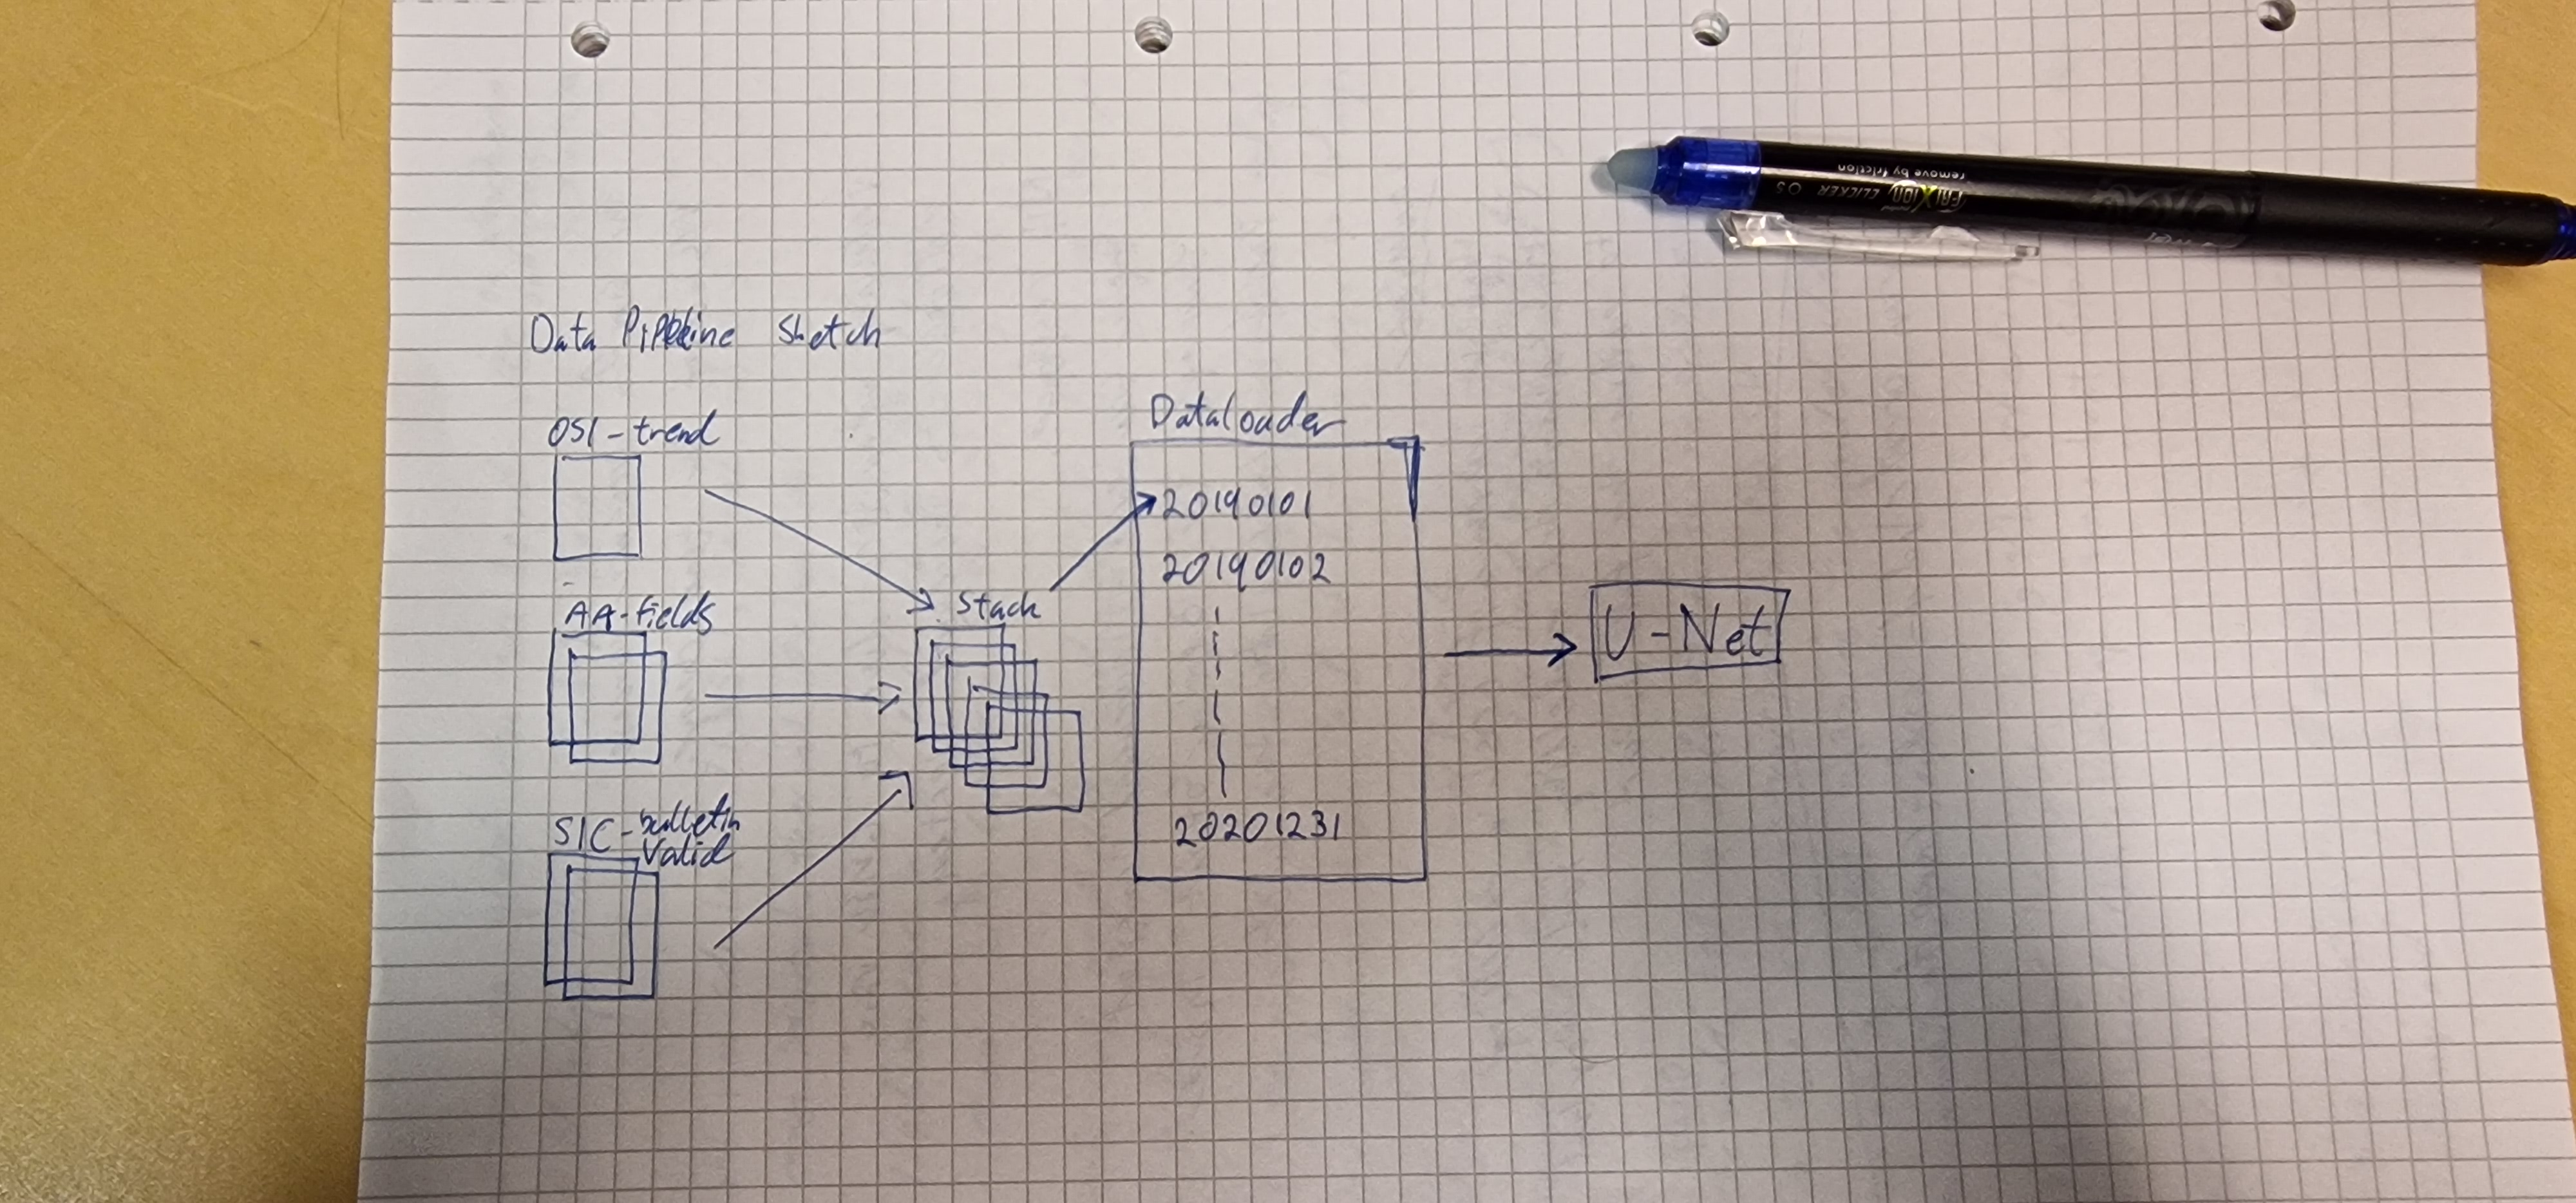
\includegraphics[width=\textwidth]{datapipeline_sketch.jpg}
    \caption{\label{fig:pipeline_sketch}Sketch showing an idealized data pipeline, where three sources are merged into one sample, kept track of by a dataloader which feeds the samples into the U-Net}
\end{figure}

\todo{This should be represented by a figure where individual sources are merged into one stack which is then treated as an entry to a dataloader which is ultimately fed into the model}

\subsection{Data sources}
Data sources used are Sea Ice charts from Nick initiated at 15:00 as well as Arome Arctic initiated at 18:00 \cite{MOI2015,Mueller2017}. For a given date, the current Ice Chart is used as a predictor for the model, while the Ice Chart drawn two days later is supplied as the model target.

\subsubsection{Sea Ice Charts}
The Sea Ice Charts used are a derived dataset of the Sea Ice Charts presented in a previous section \todo{label sections}. The present Ice Chart dataset has been postprocessed by Nick Hughes of the National Ice Service \todo{Say thanks in acknowledgements}, such that they are presented on a 1km Arome Arctic grid. Furthermore, the Ice Charts does not feature a land-mask, which has been replaced with interpolated values resulting in a spatially consistent dataset where all values present are according to the WMO Sea Ice Concentration intervals \cite{JETSI2014}. 

\subsection{AROME-Arctic}
The Arome Arctic data is structured such that the period between forecast initialization and machine learning forecast lead time is stored as a mean product in the temporal dimension at intervals [0 - 18, 42, 66]. This ensures that temporal AA information is encoded into a single field up until 12:00 UTC of the publishing date of the target ice chart. The 4d variables used from AA are T2M, uwind and vwind. Finally, the land sea mask present in AA is fetched and used as a predictor, though this land sea mask is also used for validation purposes given the case where no other SIC-product is considered.

\subsection{OSI-SAF}
A linear SIC trend of variable temporal length is computed from 12.5km OSI-SAF data \todo{Cite OSISAF}. In the case of OSI-SAF, the product is scheduled to be published daily at 15:00 UTC \todo{double check}. However, given operational concerns of the developed forecasting system, where the availability of data is essential for the model to run, the previous day OSI-SAF trend is utilized. \todo{Det er ikke sikkert det er nødvendig, hvis AA 18:00 publiseres ~19 - 20 burde OSI-SAF være publisert}.



% Local bibliography
\biblio


\end{document}